\documentclass{tufte-handout}
\usepackage{graphicx}
\graphicspath{ {./images/} }
\title{Neural Networks}
\author{Andresito Ponce}

\begin{document}
\maketitle

\begin{abstract}
	The general idea behind neural networks is to 
	maintain a \textbf{basis function} whose parameters
	can change during testing. Then the function can know 
	how to perform "better" as the testing goes on.
\end{abstract}

Previously, we had only considered a linear combination of a fixed
basis function, which usually took the form
\[ y(x, w) = f(\sum_{j=1}^{M}w_{j}\phi_{j}(x))\]

However, our goal is to make some sort of these functions depend on
certain parameters.
\[ a_{j} = \sum_{i=1}^{D}w^{(1)}_{ji}x_{i} + w^{(1)}_{j0}\]
where $a_{j}$ is the \textbf{activation} value.\footnote{Remember the
activation is the final output of this node. In classification, it 
determines which class we eventually assign to an input. The (1) 
superscript indicates they are the first layer of the NN.}

A common activation function is $y = \frac{1}{1+e^{-x}}$
We then transform the activation value by another nonlinear function
$h$, and are left with the final result $z_{j} = h(a_{j})$. 

To summarize the basic structure: supposing the result fits into 
$K$ classes, we then sum the weights of the D nodes in the first
layer and the M nodes of the second layer, and we get a formula 
in the end resembling\footnote{This equation basically says that
the final value of class $k$ is the result of adding all the nodes
from all the layers that feed into k for the two levels?}
\[ y_{k}(x, w) = \phi(\sum_{j=1}^{M}w_{kj}^{(2)}h(\sum_{i=1}^{D}
w_{ji}^{(1)}x_{i}+w_{j0}^{(1)})+w_{k0}^{(2)})\]

\subsection{Feed-Forward Neural Networks}
In this scheme, there are a set of \textbf{input nodes}, which only 
connect to the nodes on the next layer, and do not form cycles. 
There might be some \textbf{hidden layers} connected which lie between
the input layers and the final output layer. 

\begin{marginfigure}
		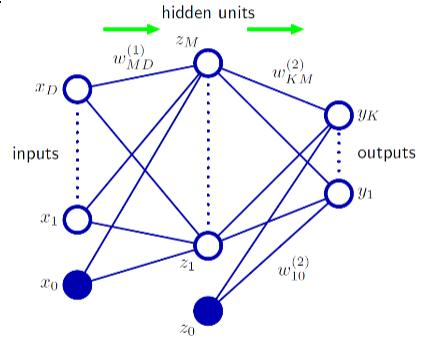
\includegraphics[scale=0.3]{neural_networks}
		\caption{The input layers feed into the hidden layers,
		the combinations of weights and basis functions can then
		determine the results of the output layers.}
\end{marginfigure}

Out of this simple model arises \textbf{deep learning}, where we have 
more than one hidden layers, \textbf{convolutional neural networks},
where nodes of one layer are not necessarily connected to the nodes
of a different layer(in contrast to multilayer perceptron).
\footnote{The lack of full connectedness means that the model is less prone to
overfit data. Instead of matrix multiplication, CNNs also use \textbf{convolution}
in at least one layer.}

For the problem of \textbf{regression}, using only one layer, we would also have to
minimize the sum of the squares between the target vector and the output of our model
$y(x, w)$. If we wanted a function with K dimensions, our final layer could have K 
output nodes, one for each dimension. 

For a classification problem, we might again use the sigmoid function to model 
our confidence of $p(C_{1}|x)$ for $p(C_{2}|x)$, by measuring the probability of one,
say $y(x,w) = p(C_{1}|x)$ and doing $1- y(x, w)$.

For multiclass classification, we can still optimize the set of weights $w$\footnote{does
this refer to optimizing for \emph{every} node in the network?} and then apply the 
\textbf{softmax} function \footnote{This would be the probs an input belongs to class K right?}
\[ y_{k}(x, w) = \frac{e^{a_{k}(x,w)}}{\sum_{j}^{}e^{a_{j}(x, w)}}\]

When utilizing gradient descent in a model such as this, we also need to calculate the gradient 
as well. Remember when looking to minimize the error function, we need to move in the direction 
where the error diminishes by the greater amount. When we calculate the derivative for the
parameters of the function, this is what we are doing. We want to move in the direction the 
error decreases the fastest.

However, under the direct approach, we would have to use all the values of the input vector. 
With \textbf{stochastic gradient descent}, we could calculate the gradient using only some values
from the input to speed up the calculation.  This would reduce the time required, especially for
large inputs. We only choose one data point to calculate the vector at a time.

\begin{marginfigure}
	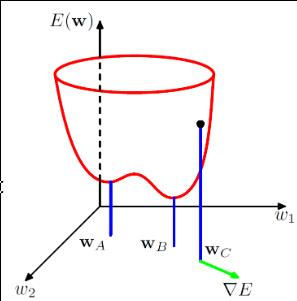
\includegraphics[scale=0.4]{gradient_descent}
	\caption{Visual description of gradient descent. We want to move 
		the weights along the derivative to the global minimum of the
		entire function space.}
\end{marginfigure}

In \textbf{gradient descent}, we want to adjust the set of weights along their derivatives. Thus,
we move always in the direction the curve is \textit{descending} the greatest. If we use sensible 
values during the calcualtion, we can avoid getting ``stuck" on a local minimum, and reach the 
absolute lowest point of a fucntion.
\section{Error Backpropagation}
The main idea behind back propagation(BP) is that we start from the last layer in our diagram, let's 
call it layer $k$. Then we travel back along the layers and along the nodes and calculate the 
error regressively along the network. Thus we \textit{propagate the error backwards}. Remember the 
basic notaion when we talk about \textit{nodes} in a neural network:\footnote{ Here, the $w$ is the 
weight, $1$ refers to the layer where we find this node, $j$ refers to the $j^{th}$ node of the 
previous layer, and i is the $i^{th}$ node of the current layer.}
\[ w^{(1)}_{ji}\]
Our main goal in BP is to calculate 
\[\frac{\partial E}{\partial w^{(2)}_{ji}}\]  
which means we want to calculate the change in the gradient relative to the weights. With this we are 
continuing our pattern of gradient descent, since we want to find the direction that minimizes the error.

If we actually go through with the partial derivatives formula, we reach that
\[ \frac{\partial E}{\partial w_{ji}} = \partial_{j}z_{i}\]
which basically means that the derivative of the gradient is just multiplying the error in node $j$
($\partial_{j}$ is the \textbf{error} here) times the $z$ value at the input of the next node.

By making use of some earlier results, we can calculate the final \textbf{backpropagation formula} as
follows:\footnote{notice $\partial k$ is from the node to which $j$ connects. Thus, by summing the 
error in the previous layer, we can basically use the same formula to calculate the error for $j$
as we did with linear regression.}
\[\partial_{j} = h'(a_{j})\sum_{k}^{}w_{kj}\partial k\]

To conclude, the steps for \textbf{backpropagation} are:
\begin{enumerate}
		\item{\textbf{Apply an input vector $x_{n}$}}. Then forward propagate through the network,
				find the activation of all the hidden units in the network.
		\item{\textbf{Find $\partial_{k}$ for the output units.}}
		\item{\textbf{Back propagate the $\partial 's$}} and obtain all the $\partial_{j}$ for all the 
				units in the network.
		\item{\textbf{Evaluate the required derivatives.}}
\end{enumerate}

\end{document}
